\documentclass{article}

% ---------------------------------------------------------------------------
% NeurIPS format. If an official NeurIPS style file is present (e.g. in the
% NeurIPS template on Overleaf), it is used. Otherwise a built-in copy of the
% NeurIPS layout is used so the file compiles anywhere.
% ---------------------------------------------------------------------------
\makeatletter
\IfFileExists{neurips_2026.sty}{\usepackage[final]{neurips_2026}\let\neurips@official\relax}{%
\IfFileExists{neurips_2025.sty}{\usepackage[final]{neurips_2025}\let\neurips@official\relax}{%
\IfFileExists{neurips_2024.sty}{\usepackage[final]{neurips_2024}\let\neurips@official\relax}{}}}
\ifdefined\neurips@official\else
  % --- built-in NeurIPS layout: 5.5in x 9in text, Times 10pt, no indent ---
  \usepackage[letterpaper,textwidth=5.5in,textheight=9in,top=1in,
    headheight=12pt,headsep=25pt,footskip=30pt]{geometry}
  \usepackage{times}
  \setlength{\parindent}{0pt}
  \setlength{\parskip}{5.5pt}
  \renewcommand{\@maketitle}{%
    \vbox{\hsize\textwidth\linewidth\hsize
      \vskip 0.1in
      \hrule height 4pt \vskip 0.25in \vskip -\parskip
      \centering{\LARGE\bf \@title\par}
      \vskip 0.29in \vskip -\parskip
      \hrule height 1pt \vskip 0.09in
      \def\And{\end{tabular}\hfil\linebreak[0]\hfil\begin{tabular}[t]{c}\bf\rule{\z@}{24pt}\ignorespaces}%
      \begin{tabular}[t]{c}\bf\rule{\z@}{24pt}\@author\end{tabular}%
      \vskip 0.3in \vskip -\parskip}}
  \renewenvironment{abstract}{%
    \centerline{\large\bf Abstract}\vspace{0.5ex}%
    \begin{quote}\setlength{\parskip}{0pt}}{\par\end{quote}\vskip 1ex}
  \renewcommand{\section}{\@startsection{section}{1}{\z@}%
    {-2.0ex \@plus -0.5ex \@minus -0.2ex}{1.5ex \@plus 0.3ex \@minus 0.2ex}%
    {\large\bf\raggedright}}
  \renewcommand{\subsection}{\@startsection{subsection}{2}{\z@}%
    {-1.8ex \@plus -0.5ex \@minus -0.2ex}{0.8ex \@plus 0.2ex}%
    {\normalsize\bf\raggedright}}
  \renewcommand{\paragraph}{\@startsection{paragraph}{4}{\z@}%
    {1.5ex \@plus 0.5ex \@minus 0.2ex}{-1em}{\normalsize\bf}}
  \usepackage{caption}
  \captionsetup{font=small}
\fi
\makeatother
\usepackage[T1]{fontenc}
\usepackage[utf8]{inputenc}
\usepackage{amsmath,amssymb}
\usepackage{booktabs}
\usepackage{microtype}
\usepackage{xcolor}
\usepackage{tikz}
\usepackage{pgfplots}
\pgfplotsset{compat=1.17}
\usepackage[hidelinks]{hyperref}

\definecolor{series1}{HTML}{2A78D6}  % data
\definecolor{series2}{HTML}{EB6834}  % reference / theory
\definecolor{inkmuted}{HTML}{52514E}

\pgfplotsset{
  every axis/.append style={
    axis line style={inkmuted},
    tick style={inkmuted},
    tick label style={font=\scriptsize},
    label style={font=\footnotesize},
    title style={font=\footnotesize},
    legend style={font=\scriptsize, draw=none, fill=white, fill opacity=0.85, text opacity=1},
    legend cell align=left,
    ymajorgrids, grid style={gray!20},
  },
}

\newcommand{\code}[1]{\texttt{#1}}
\newcommand{\peter}{Peter}
\newcommand{\pbj}{PB\&J}

\title{All You Need is Peter to Beat PB\&J}
\author{Shawn Wang, David Yu, Kevin Pyo, Brian Gasca, Daniel Wu \\
\normalfont CSE 150A Final Project}
\date{}

\begin{document}
\maketitle

% ===========================================================================
\begin{abstract}
Kuhn poker is a three-card version of poker whose optimal (Nash equilibrium)
strategy is known exactly. At equilibrium, player one expects to lose $1/18$
of a chip per hand~\cite{wiki}. We ask how close a learning agent can get to
that optimum, and we answer in three stages that follow how our code evolved.
(1) With player two (\pbj) fixed at equilibrium, we maximize player one's
(\peter's) exact expected value (EV) over four probabilities by hill climbing.
All 10{,}000 restarts reach $-1/18$, but three of the four probabilities never
move, so the learned strategies lose an extra $0.19$ chips per hand to a best
counter-strategy. (2) A tabular Q-learner that sees only sampled chips finds the
same best responses against five versions of \pbj{} in at most $100{,}000$
hands, and escapes a local optimum that traps hill climbing. (3) Finally both
players learn only from their own winnings. Using an exact evaluator built on
Bayes' rule over the hidden card, we measure \emph{exploitability}, the
distance from equilibrium. Naive self-play and fictitious self-play with
Q-learned replies cut it from $0.458$ to about $0.04$ chips per hand but then
plateau, even with $10\times$ more hands; fictitious play with exact replies
keeps falling to $0.006$. Learning the optimal \emph{value} is easy; learning
the optimal \emph{strategy} needs both players to adapt and accurate replies.
\end{abstract}

% ===========================================================================
\section{Problem Description}

In poker you never see your opponent's cards, so every decision is made under
uncertainty. Our project asks: ``How close can a learning agent get to the
theoretically optimal poker strategy?'' Real poker is far too large to solve
exactly, so there is no optimal strategy to compare against. We therefore use
\textbf{Kuhn poker}, a minimal version that still has hidden cards, betting and
bluffing, and whose optimal strategy is known~\cite{wiki,kuhn1950}. Because
the answer is known, we can measure exactly how far a learned strategy is from
optimal.

\paragraph{Relevance to probabilistic reasoning.} Kuhn poker is a small
probabilistic model with a hidden variable, the opponent's card. A good player
has to reason about the probability of each opponent card given the
opponent's actions, which is Bayes' rule. Once the opponent's strategy is
fixed, the game becomes a single-agent decision problem (an MDP) for the
learner, and its expected value can be computed exactly by enumeration or
estimated by sampling. That lets us compare exact and approximate inference
on the same problem.

\paragraph{Rules.} The deck has three cards, Jack $<$ Queen $<$ King. Each
player antes one chip (starting money placed in the pot before the deal) and
gets one private card; the third card is put aside unseen. The first player
checks or bets one chip. After a check, the second player can check, which
goes to a showdown, or bet; the first player must then call or fold. After a
bet, the second player calls (showdown) or folds. At a showdown the higher card
wins the pot.

\paragraph{Naming conventions.} \textbf{\peter} is player one (acts first);
\textbf{\pbj} is player two. \code{bet\_J}, \code{bet\_Q}, \code{bet\_K} are
\peter's chances of betting first with a Jack, Queen or King (checking is the
complement), and \code{call\_Q} is his chance of calling after checking a Queen
into a bet. $q$ is \pbj's bluffing and calling probability, $\alpha$ indexes
\peter's optimal strategies, \code{lr} is the hill-climbing step size, $M$ the
number of simulated hands, and $\epsilon$ the exploration rate.

\paragraph{The optimal strategy.} At equilibrium, \peter{} expects to lose
$1/18 \approx 0.0556$ chips per hand~\cite{wiki}. \pbj{} has one equilibrium
strategy. With a King, \pbj{} always bets or calls. With a Queen, \pbj{}
checks, and calls a bet with probability $q = 1/3$. With a Jack, \pbj{} never
calls, and bluffs (bets after a check) with probability $q = 1/3$. \peter's
optimal strategy is not a single value but a range indexed by
$\alpha$~\cite{wiki,kuhn1950}:
\begin{equation}
  \code{bet\_J} = \alpha, \quad \code{bet\_Q} = 0, \quad
  \code{bet\_K} = 3\alpha, \quad \code{call\_Q} = \alpha + \tfrac13.
  \label{eq:equilibrium}
\end{equation}

% ===========================================================================
\section{Data Sourcing and Processing}

\paragraph{Source.} There is no external dataset. All data are generated
from the rules of the game. Each data point is a \emph{deal}, an ordered pair
of distinct cards for \peter{} and \pbj{}. The six possible deals are equally
likely ($1/6$ each). Everything else that happens in a hand is drawn from the
two players' strategies. We use this data in two ways. For the exact EV, we
enumerate all six deals and every branch of the betting tree. For
verification, we simulate $M$ random hands. The stage-1 run (\code{logic.py})
repeated the full pipeline from 10{,}000 random starts and wrote each run's
learned probabilities and simulated EV to \code{log.txt}. For stages 2 and 3
the sampled hands \emph{are} the training data: every learner sees one dealt
hand at a time and only its own card, its actions and the chips won. We use
seeds 0--9 for every sampled configuration and freeze each run's policy after
$10^3$, $10^4$, $10^5$ and $10^6$ hands; \code{experiments/run\_experiments.py}
writes every checkpoint to JSON logs in \code{experiments/logs/}.

\paragraph{Processing and feature selection.} Simulated data has no missing
values or noise to clean, so our processing is about choosing the right
variables:
\begin{itemize}\itemsep0pt
  \item \textbf{One variable per card, not per deal.} Our first design used six
  variables, one per dealt pair, searched with six nested \code{while} loops. A
  variable tied to a pair of cards can ``look into'' \pbj's hidden card, which
  \peter{} cannot see, and pairs that share \peter's card were forced to
  interact. The results were inaccurate and skewed. Indexing by \peter's own
  card fixes this, because it matches what \peter{} actually observes.
  \item \textbf{Dropping dominated actions.} \peter{} always folds a Jack when
  facing a bet, since a Jack can never win a showdown. He always calls with a
  King, since a King can never lose one. Fixing these leaves four free
  variables.
\end{itemize}

% ===========================================================================
\section{Modeling and Inference}
\label{sec:model}

\begin{figure}[htb]
\centering
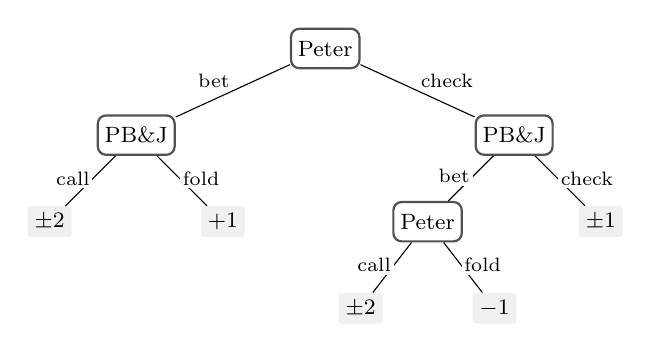
\begin{tikzpicture}[
  level distance=11mm,
  every node/.style={font=\footnotesize},
  dec/.style={rectangle, rounded corners=3pt, draw=inkmuted, thick, inner sep=2.5pt, minimum height=5mm},
  leaf/.style={rectangle, rounded corners=1pt, fill=gray!12, inner sep=2.5pt},
  lbl/.style={font=\scriptsize, fill=white, inner sep=1pt},
  level 1/.style={sibling distance=48mm},
  level 2/.style={sibling distance=22mm},
  level 3/.style={sibling distance=17mm},
]
\node[dec] {\peter}
  child { node[dec] {\pbj}
    child { node[leaf] {$\pm2$} edge from parent node[lbl, left, pos=0.45] {call} }
    child { node[leaf] {$+1$} edge from parent node[lbl, right, pos=0.45] {fold} }
    edge from parent node[lbl, above left] {bet} }
  child { node[dec] {\pbj}
    child { node[dec] {\peter}
      child { node[leaf] {$\pm2$} edge from parent node[lbl, left, pos=0.45] {call} }
      child { node[leaf] {$-1$} edge from parent node[lbl, right, pos=0.45] {fold} }
      edge from parent node[lbl, left, pos=0.45] {bet} }
    child { node[leaf] {$\pm1$} edge from parent node[lbl, right, pos=0.45] {check} }
    edge from parent node[lbl, above right] {check} };
\end{tikzpicture}
\caption{Betting tree for one hand, with \peter's net chips at each end. $\pm$
means \peter{} wins if he holds the higher card and loses otherwise.}
\label{fig:tree}
\end{figure}

\paragraph{Shared model.} Kuhn poker is a two-player zero-sum game with
imperfect information. A player's state is an \emph{information set}: their own
card plus the betting so far (six per player). Actions are bet/check or
call/fold, and the reward is the net chips won at the end of the hand
(Figure~\ref{fig:tree}). Assumptions: (1) \peter{} always acts first; (2) each
player sees only their own card, so a strategy is one betting probability per
information set; (3) the deal is uniform over the six ordered pairs; (4) the
showdown depends on both cards. When one player's strategy is held fixed, that
player becomes part of the environment and the game is a single-agent MDP over
the other player's information sets. Stages 1 and 2 use this reduction;
stage 3 drops it.

\paragraph{Inference about the hidden card.} The opponent's card is a hidden
variable. Given the opponent's strategy, the posterior over it follows Bayes'
rule, $P(c \mid \text{actions}) \propto P(\text{actions} \mid c)\,P(c)$. For
example, if \peter{} checks a Queen and \pbj{} bets, \pbj{} holds the King
with probability $\frac{1 \cdot 1/2}{1\cdot 1/2 + \frac13 \cdot 1/2} = 3/4$.

\paragraph{Exact evaluation and exploitability.} Our evaluator
(\code{evaluate.py}) enumerates the six deals and every branch of
Figure~\ref{fig:tree}, replacing each coin flip by its probability, so it
returns exact EVs with no sampling noise. Working backward through the tree
with the posterior above, it also finds each player's exact \emph{best
response} to a fixed opponent. We verified it against brute force over all 64
deterministic strategies per player and against OpenSpiel's Kuhn
poker~\cite{openspiel}. For a strategy pair $(\pi_1, \pi_2)$, the
exploitability is half the total amount the two players could gain by switching
to their best responses,
\[
  \text{expl}(\pi_1,\pi_2) = \tfrac12\big[\max_{\pi_1'} v(\pi_1',\pi_2) - \min_{\pi_2'} v(\pi_1,\pi_2')\big],
\]
where $v$ is \peter's EV. It is $0$ exactly at a Nash equilibrium. Exact
evaluation is used only to \emph{score} frozen policies in stages 2--3; the
learners there never see it.

\begin{table}[tb]
\centering
\small
\caption{How the learner evolved. ``Learns from'' is what the algorithm uses.}
\label{tab:stages}
\setlength{\tabcolsep}{4pt}
\begin{tabular}{llll}
\toprule
Stage (code) & Parameters & Learns from & Target \\
\midrule
1 Hill climbing (\code{logic.py}) & 4 probabilities & exact EV (\pbj{} known) & best response \\
2 Partial Q-learning (\code{partial\_q\_learning.py}) & 8 Q-values & sampled chips & best response \\
3 Self-play (\code{q\_learning.py}, \code{self\_play.py}) & 12 Q-values/player & own chips & equilibrium \\
\bottomrule
\end{tabular}
\end{table}

\subsection{Stage 1: optimizing against a fixed strategy toward a known EV}
Our first version assumes \pbj's strategy is known and fixed (with parameter
$q$), so \peter's exact EV is a closed-form function of his four
probabilities. We maximize it by \emph{coordinate hill climbing}: from a random
start, nudge each probability up or down by $\code{lr} = 0.005$ and keep a
change only if it strictly raises the EV; stop when no nudge helps (at most
1000 sweeps). We then check the EV with a Monte Carlo simulation of
$M = 200{,}000$ hands. This is planning with a known model, not learning from
experience, and its target is a known number ($-1/18$ at $q = 1/3$).

\subsection{Stage 2: partial Q-learning (4 decision points)}
Stage 2 removes the exact EV: \peter{} learns only from the chips won in
sampled hands, which is model-free reinforcement learning. The states are
\peter's four non-trivial information sets, $(c, \text{start})$ for each card
$c$ with actions bet/check, and (Queen, facing a bet) with call/fold, for
8 Q-values. A Jack facing a bet always folds and a King always calls, since
those choices are dominated. After each hand, every visited pair is updated
toward its target,
\[
  Q(s,a) \leftarrow Q(s,a) + \tfrac{1}{N(s,a)}\big[y - Q(s,a)\big],\qquad
  y = \begin{cases} r & \text{last decision of the hand,} \\
  \max_{a'} Q(s', a') & \text{otherwise,} \end{cases}
\]
where $r$ is the chips won, $N(s,a)$ the visit count, and $s'$ = (Queen,
facing a bet) after \peter{} checks a Queen and \pbj{} bets; there is no
discounting. Actions are $\epsilon$-greedy ($\epsilon = 0.1$). The
learned strategy is the greedy policy, which is pure (each probability is 0
or 1). \pbj{} is still fixed, so the target is still a best response.

\subsection{Stage 3: each player learns from their own winnings}
Stage 3 makes both players learners, as in our proposal. Each player has a
Q-table over all six of its information sets (12 Q-values), with the same
update rule, $\epsilon = 0.2$, and reward equal to its own net chips (\pbj{}
receives the negative of \peter's). Nothing is forced or hard-coded. We test
four set-ups. \textbf{Fixed opponents:} \peter{} learns against four fixed
bots (always-pass, always-bet, uniformly random, equilibrium), to separate
exploiting a bot from playing well. \textbf{Naive self-play:} both players
learn at the same time from the same hands. Because a greedy policy is pure, it
cannot bluff at a mixed rate, so we also track each player's \emph{average}
strategy over time. \textbf{Fictitious self-play, learned replies:} in each
round, each player trains a fresh Q-learner for 500 hands against the
opponent's frozen \emph{average} strategy, then adds that reply to its own
average~\cite{heinrich2015}. Averaging over replies is what lets a sequence of
pure strategies approach a mixed equilibrium; fictitious play is known to
converge in two-player zero-sum games. \textbf{Fictitious play, exact
replies:} the same loop with each reply computed exactly by the evaluator,
used as a model-based reference with no sampling. One round of the sampled
methods uses 1{,}000 hands; we run 1{,}000 rounds ($10^6$ hands).
% ===========================================================================
\section{Results and Discussion}

\subsection{Stage 1: hill climbing configurations}

\begin{table}[tb]
\centering
\small
\caption{Stage 1 against \pbj{} with parameter $q$ ($\code{lr} = 0.005$,
1{,}000 random starts each). EV is \peter's exact EV after hill climbing.}
\label{tab:configs}
\begin{tabular}{llll}
\toprule
Setting & Final EV & Learned strategy & Cost / stability \\
\midrule
$q = 0$  & $+1/6$  & \code{bet\_J}$=1$, \code{call\_Q}$=0$ & all runs agree \\
$q = 0.2$ & $+1/30$ & \code{bet\_J}$=1$, \code{call\_Q}$=0$ & all runs agree \\
$q = 1/3$ (optimal) & $-1/18$ & only \code{bet\_Q}$=0$ & 3 of 4 stay random \\
$q = 0.5$ & $0$ & \code{bet\_J}$=0$, \code{call\_Q}$=1$ & all runs agree \\
$q = 1$   & $+1/6$ or $0$ & \code{bet\_J}$=0$ & 13.5\% stuck at $0$ \\
\bottomrule
\end{tabular}
\end{table}

\paragraph{Learning rate.} With $\code{lr} \in \{0.001, 0.005, 0.02, 0.1\}$
(1{,}000 starts each, $q = 1/3$), every run reached $-1/18$ with
$\code{bet\_Q} = 0$. A larger \code{lr} only made training faster, roughly in
proportion: from about 4{,}000 EV evaluations per run at $0.001$ down to about
50 at $0.1$. The
reason is that the EV changes only through \code{bet\_Q}, and in a straight
line (Section~\ref{sec:quant}), so step size affects speed but not the result.

\paragraph{\pbj's strategy $q$.} This was the most informative comparison.
When \pbj{} deviates from $q = 1/3$, \peter{} learns to exploit it and wins
chips. With $q$ too low (\pbj{} bluffs and calls too rarely), \peter{} always
bluffs with a Jack and never calls with a Queen. With $q$ too high, he does the
reverse. Only at $q = 1/3$ is \peter{} held to his lowest EV, $-1/18$, which
confirms that $q = 1/3$ is \pbj's optimal strategy. \code{bet\_K} stayed random
for every $q$. \pbj{} calls with a Queen exactly as often as it bluffs with a
Jack (both $q$), so \peter's King earns the same whether he bets or checks. At
$q = 1$, 13.5\% of runs got stuck at an EV of $0$ instead of $1/6$. These runs
always bet the Queen and had a low \code{call\_Q}. Checking a Queen only pays
off if \peter{} then calls, so lowering \code{bet\_Q} alone made things worse.
Raising \code{call\_Q} alone changed nothing, because \peter{} never checked a
Queen. Changing one variable at a time cannot escape this local optimum.

\subsection{Stage 1: quantitative results}
\label{sec:quant}

All 10{,}000 logged runs reached an exact EV of $-1/18$. Table~\ref{tab:indiff}
explains why. Against \pbj, \peter{} gets the same EV whatever he does, except
when he bets with a Queen. Adding up the rows gives
\[
  \text{EV} = -\frac{1 + \code{bet\_Q}}{18},
\]
so the best \peter{} can do is to set $\code{bet\_Q} = 0$, and every run
found it.

\begin{table}[htb]
\centering
\small
\caption{\peter's EV for each action, by card, against \pbj.}
\label{tab:indiff}
\setlength{\tabcolsep}{4pt}
\begin{tabular}{lccc}
\toprule
Card & If bet & If check & Share of total EV \\
\midrule
Jack  & $-1$   & $-1$   & $-1/3$ \\
Queen & $-1/2$ & $-1/3$ & $-1/9 - \code{bet\_Q}/18$ \\
King  & $7/6$  & $7/6$  & $+7/18$ \\
\midrule
Total & & & $-(1 + \code{bet\_Q})/18$ \\
\bottomrule
\end{tabular}
\end{table}

Appendix~\ref{app:sim} shows that the simulated EVs agree with the exact
value to within ordinary sampling noise ($\approx 0.003$ per run).

\subsection{Stage 1: qualitative insights}
\label{sec:qual}



\paragraph{What the model captures.} The model captures the probabilistic
reasoning behind the equilibrium. If \peter{} checks a Queen and \pbj{} bets,
\pbj{} holds the King $3/4$ of the time (Section~\ref{sec:model}), so
calling and folding both average $-1$ chip, which is exactly why
\code{call\_Q} does not matter against \pbj. \pbj's bluffing rate of $1/3$ is
chosen to make \peter{} indifferent in this way.

\paragraph{What the model misses.} Only \code{bet\_Q} matched the equilibrium
(Table~\ref{tab:params}, Appendix~\ref{app:strategy}). The other three probabilities look exactly like
uniform random numbers. They have no effect on the EV, so the hill climber
never accepted a change to them, and they stayed at their random starting
values. Figure~\ref{fig:strategy}a shows that \code{bet\_J} and \code{bet\_K}
are scattered across the whole square instead of lying on the equilibrium
line. Only 1.3\% of runs came within $0.1$ of an equilibrium strategy for some
$\alpha$. This matters because a real opponent would not stay fixed. If \pbj{}
switched to its best counter-strategy, it would win an extra $0.19$ chips per
hand on average from \peter's learned strategies (Figure~\ref{fig:strategy}b),
more than three times the equilibrium value itself. Our proposal expected
this when training against a fixed opponent: the learner exploits that
opponent well but can itself be exploited.

\subsection{Stage 1: convergence and scalability}

Every run converged within at most 200 productive sweeps; the only
instability was the local optimum at $q = 1$. Almost all of the cost is the
verification simulation (about 11 minutes for the 10{,}000-run log). More
restarts or simulated hands would not change the learned strategy, because the
gap to the equilibrium comes from the objective, not from noise. Exact
enumeration also needs \pbj's strategy and does not scale to real poker,
which motivates the model-free stages below.

\subsection{Stage 2: partial Q-learning}

\begin{table}[tb]
\centering
\small
\caption{Learning a best response to a fixed opponent. Number of the 10 seeds
whose frozen greedy policy is an exact best response after $10^3$--$10^6$
training hands, and the median EV of the $10^6$-hand policy against the
opponent's best counter-strategy (worst case).}
\label{tab:stage2}
\setlength{\tabcolsep}{4.5pt}
\begin{tabular}{lcccccc}
\toprule
Opponent & Best EV & $10^3$ & $10^4$ & $10^5$ & $10^6$ & Worst-case EV \\
\midrule
\multicolumn{7}{l}{\emph{Stage 2: partial Q-learning vs.\ \pbj{} with parameter $q$}} \\
$q = 0$ & $+1/6$ & 10/10 & 10/10 & 10/10 & 10/10 & $-1/2$ \\
$q = 0.2$ & $+1/30$ & 7/10 & 10/10 & 10/10 & 10/10 & $-1/2$ \\
$q = 1/3$ & $-1/18$ & 10/10 & 10/10 & 10/10 & 10/10 & $-1/4$ \\
$q = 0.5$ & $0$ & 6/10 & 10/10 & 10/10 & 10/10 & $-1/6$ \\
$q = 1$ & $+1/6$ & 7/10 & 9/10 & 10/10 & 10/10 & $-1/6$ \\
\midrule
\multicolumn{7}{l}{\emph{Stage 3: Q-learning over all six information sets vs.\ fixed bots}} \\
always-pass & $+1$ & 10/10 & 10/10 & 10/10 & 10/10 & $-1/2$ \\
always-bet & $+1/3$ & 10/10 & 10/10 & 10/10 & 10/10 & $-1/6$ \\
random & $+1/2$ & 10/10 & 10/10 & 10/10 & 10/10 & $-1/3$ \\
equilibrium & $-1/18$ & 7/10 & 10/10 & 10/10 & 10/10 & $-1/6$ \\
\bottomrule
\end{tabular}
\end{table}

Without ever seeing \pbj's strategy, the Q-learner found the same best
responses as hill climbing (Table~\ref{tab:stage2}). After $10^3$ hands 40 of
50 runs were already optimal, after $10^4$ hands 49 of 50, and after $10^5$
hands all 50. The one run still wrong at $10^4$ hands ($q = 1$) kept betting
its Queen, the same trap that held 13.5\% of hill-climbing runs at an EV of
$0$. Exploration makes \peter{} sometimes check a Queen anyway, so he learns
that calling afterward pays, and the run escaped by $10^5$ hands. This is the
coordinated change that one-variable-at-a-time hill climbing cannot make.
Q-learning also shows the same flat directions: at $q = 1/3$ the greedy
\code{bet\_J}, \code{bet\_K} and \code{call\_Q} differ from seed to seed,
because their two Q-values are truly tied and only noise picks a winner
(e.g.\ 1.161 vs.\ 1.168 for betting vs.\ checking a King in seed 0). More hands do not
fix this: the gap is exactly zero. As a result, the worst-case EV of the
learned policies ranges from $-1/2$ to $-1/6$, far below $-1/18$. The cost of
dropping the model is data: about $10^4$--$10^5$ sampled hands instead of a
few hundred exact EV evaluations.

\subsection{Stage 3: learning against fixed opponents}

With nothing hard-coded, the learner still reached an exact best response to
every bot in every seed by $10^4$ hands (Table~\ref{tab:stage2}, bottom). Learning to
exploit a bot, however, is not learning to play well. Against always-pass,
\peter{} learns to bet his Jack and Queen (with a King, betting and checking both win) and collects the maximum $+1$ chip per hand, but
that same policy loses $1/2$ per hand to a best counter-strategy, nine times
worse than the equilibrium value. Even the policies trained against the
equilibrium bot lose $1/6$ to $1/2$ against their counter-strategy. A best
response to a fixed opponent is pure and ignores how the opponent could
adapt, which is why stage 3 lets both players learn.

\subsection{Stage 3: self-play}

\begin{figure}[tb]
\centering
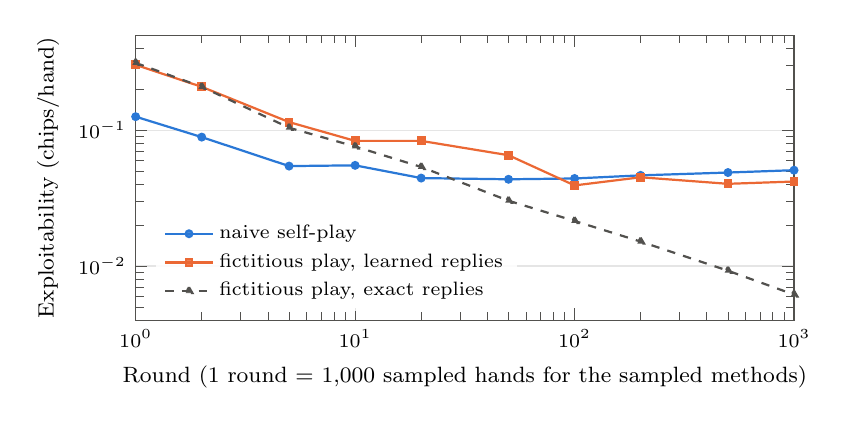
\begin{tikzpicture}
\begin{axis}[
  width=0.82\linewidth, height=5.2cm,
  xmode=log, ymode=log,
  xlabel={Round (1 round $=$ 1{,}000 sampled hands for the sampled methods)},
  ylabel={Exploitability (chips/hand)},
  xmin=1, xmax=1000, ymin=0.004, ymax=0.5,
  legend pos=south west,
]
\addplot[series1, thick, mark=*, mark size=1.2pt] coordinates {(1,0.12559) (2,0.08883) (5,0.05437) (10,0.05505) (20,0.04437) (50,0.04347) (100,0.04407) (200,0.04646) (500,0.04873) (1000,0.05071)};
\addlegendentry{naive self-play}
\addplot[series2, thick, mark=square*, mark size=1.2pt] coordinates {(1,0.30208) (2,0.20833) (5,0.11458) (10,0.08333) (20,0.08333) (50,0.06536) (100,0.03919) (200,0.04498) (500,0.04025) (1000,0.04185)};
\addlegendentry{fictitious play, learned replies}
\addplot[inkmuted, thick, dashed, mark=triangle*, mark size=1.4pt] coordinates {(1,0.31250) (2,0.20833) (5,0.10417) (10,0.07576) (20,0.05357) (50,0.03023) (100,0.02145) (200,0.01513) (500,0.00923) (1000,0.00616)};
\addlegendentry{fictitious play, exact replies}
\end{axis}
\end{tikzpicture}
\caption{Exploitability of the players' \emph{average} strategies (median of
10 seeds for the sampled methods; the exact method is deterministic). The
uniform starting pair has exploitability $0.458$; $0$ is a Nash equilibrium.}
\label{fig:selfplay}
\end{figure}

Figure~\ref{fig:selfplay} answers our main question. Both model-free
self-play methods cut exploitability by a factor of about ten, from $0.458$ to
$0.044$ (naive) and $0.039$ (learned replies) chips per hand after $10^5$
hands. Then they stop improving: ten times more hands left them at $0.051$ and
$0.042$, with every seed between $0.035$ and $0.054$.
The exact-reply version keeps falling steadily, to $0.006$ after 1{,}000
rounds. Since the two fictitious-play versions differ only in how each reply
is computed, the plateau comes from the \emph{replies}, not from too few hands.
Each learned reply is trained for only 500 hands with $\epsilon = 0.2$, so
some replies are wrong, and wrong replies keep entering the average at a fixed
rate. Naive self-play has no convergence guarantee at all; its players keep
chasing each other's latest pure policy. In every method the \emph{current}
greedy pair stays far from equilibrium (0.17--0.42), because equilibrium play
requires mixing, such as bluffing a Jack only some of the time, and a greedy
policy cannot mix. Only the average strategy approaches the equilibrium.

\paragraph{How many hands are enough?} For learning a best response to a fixed
opponent, $10^4$ hands sufficed in 89 of 90 runs (stages 2 and 3) and $10^5$
in all of them. For approaching the equilibrium, $10^5$ hands brought the
sampled methods to their plateau, and more data alone does not help. The
next improvement has to come from the algorithm: training each reply longer as
rounds go on, decaying $\epsilon$, or methods such as counterfactual regret
minimization. Compute was not the bottleneck: all $1.1\times10^8$ training
hands of stages 2 and 3 took under two minutes on a laptop.

% ===========================================================================
\section{Conclusion}

We asked how close a learning agent can get to optimal Kuhn poker, and
answered in three stages. (1) Hill climbing on the exact EV against a fixed
equilibrium \pbj{} reached the optimal value $-1/18$ in all 10{,}000 runs,
but not the optimal strategy: three of four probabilities never moved.
(2) Partial Q-learning, using only sampled chips, found the same best
responses against five versions of \pbj{} within $10^5$ hands and escaped the
local optimum that trapped hill climbing. (3) With both players learning only
from their own winnings, self-play and fictitious play with Q-learned replies
cut exploitability from $0.458$ to about $0.04$ chips per hand, while
fictitious play with exact replies reached $0.006$. Choosing variables that
use only what a player can see (their own card and the betting) was what made
every stage correct.

\paragraph{Limitations.} Best responses to a fixed opponent are pure and
exploitable, however exact (stages 1--2 and the fixed-opponent runs lose
$1/6$ to $1/2$ chip per hand to a counter-strategy). Greedy Q-learning
policies cannot mix, so only \emph{averaged} strategies approach equilibrium,
and with fixed-length learned replies the sampled methods plateau near $0.04$
instead of converging. Our results also rely on a game small enough to
evaluate exactly; exploitability cannot be computed this way for real poker.

\paragraph{Extensions.} Train each fictitious-play reply longer as rounds go
on and decay $\epsilon$, which should let the learned-reply version follow the
exact one toward $0$; compare with counterfactual regret minimization; and move
on to three-player Kuhn poker~\cite{wiki,szafron2013}. As the professor says:
all models are wrong but some are useful.

% ===========================================================================
\section{Reflections \& Contributions}

\paragraph{Advice for future students.} Check early that every variable in
your model only uses information the agent can actually see; our first
six-variable design did not, and it skewed every result. Compute exact answers
whenever the problem is small enough, and use simulation as a check rather
than the main tool. Finally, matching the right \emph{number} does not mean the
model learned the right \emph{behavior}, so look at the learned parameters, not
just the score.

\paragraph{Contributions and individual reflections.}
\begin{itemize}\itemsep2pt
  \item \textbf{Shawn Wang:} Brainstormed ideas, did background research into kuhn poker's logic system, and created beta versions of the RL algorithm. \emph{Reflection:} I think that reverse engineering this problem was actually harder than it would have been to just start from scratch and use a brute force compute. However, I learned it was much more rewarding to understand the underlying probability logic in order to reduce compute power needed to solve the problem. On top of saving a couple magnitudes of compute power we also got to work through kuhn poker like engineers, poking around and examining probability branches to find where we could optimize.
  \item \textbf{David Yu:} Helped with brainstorming ideas and added Q-Learning comparison to the writeup. \emph{Reflection:} I learned about poker, particularly Kuhn Poker. I also learned that some decisions have obvious answer and don't need to be learned(ie a king facing a bet should call), this shrinks the q table from 12 to 8 values.
  \item \textbf{Kevin Pyo:} [1--2 sentences on tasks]. \emph{Reflection:} [what you learned].
  \item \textbf{Brian Gasca:} [1--2 sentences on tasks]. \emph{Reflection:} [what you learned].
  \item \textbf{Daniel Wu:} [1--2 sentences on tasks]. \emph{Reflection:} [what you learned].
\end{itemize}

\paragraph{Use of generative AI.} 
% What you guys feel
We used Claude to help draft and format this report in LaTeX and to run the additional configuration experiments in Table~\ref{tab:configs} with our own \code{logic.py} functions. We also used Claude to restructure Sections~3--5 around the three stages, and to write and run the scripts in \code{experiments/}, which only loop over seeds and settings, call our existing learners and score them with \code{evaluate.py}; the raw logs are in \code{experiments/logs/}. All modeling decisions, code and final content were reviewed and verified by the team. Additionally, all iterations of LLM generated code were based on handwritten code given as input so that the baseline logic remained the same throughout iterations.



% ===========================================================================
\section{References}
{\renewcommand{\section}[2]{}%
\begin{thebibliography}{9}
\small
\bibitem{wiki}
``Kuhn poker,'' \emph{Wikipedia}.
\url{https://en.wikipedia.org/wiki/Kuhn_poker}

\bibitem{kuhn1950}
H.~W. Kuhn, ``Simplified two-person poker,'' in H.~W. Kuhn and A.~W. Tucker
(eds.), \emph{Contributions to the Theory of Games}, vol.~1, Princeton
University Press, 1950, pp.~97--103. (Cited by~\cite{wiki}.)

\bibitem{szafron2013}
D.~Szafron, R.~Gibson, and N.~Sturtevant, ``A parameterized family of
equilibrium profiles for three-player Kuhn poker,'' in \emph{Proc.\ 12th Int.\
Conf.\ on Autonomous Agents and Multiagent Systems (AAMAS)}, 2013. (Cited
by~\cite{wiki}.)

\bibitem{heinrich2015}
J.~Heinrich, M.~Lanctot, and D.~Silver, ``Fictitious self-play in
extensive-form games,'' in \emph{Proc.\ 32nd Int.\ Conf.\ on Machine Learning
(ICML)}, 2015, pp.~805--813.

\bibitem{openspiel}
M.~Lanctot \emph{et al.}, ``OpenSpiel: A framework for reinforcement learning
in games,'' arXiv:1908.09453, 2019.
\end{thebibliography}}


\appendix
\section{Stage 1: simulation check}
\label{app:sim}

The stage-1 log rounds probabilities to three decimals and stores only the
simulated EV; for the analysis we recomputed each run's exact EV from the
logged probabilities.

\paragraph{Simulated hands $M$.} Repeated simulations of one equilibrium
strategy ($\alpha = 0.2$) give an RMS error in the simulated EV of $0.039$,
$0.013$, $0.0037$ and $0.0034$ for $M = 10^3$, $10^4$, $10^5$ and
$2\times10^5$ hands (0.3, 3, 36 and 67\,ms per run). The error shrinks like
$1/\sqrt{M}$, so ten times more hands buys about three times more accuracy.

\begin{figure}[tb]
\centering
\begin{minipage}[t]{0.48\linewidth}
\centering
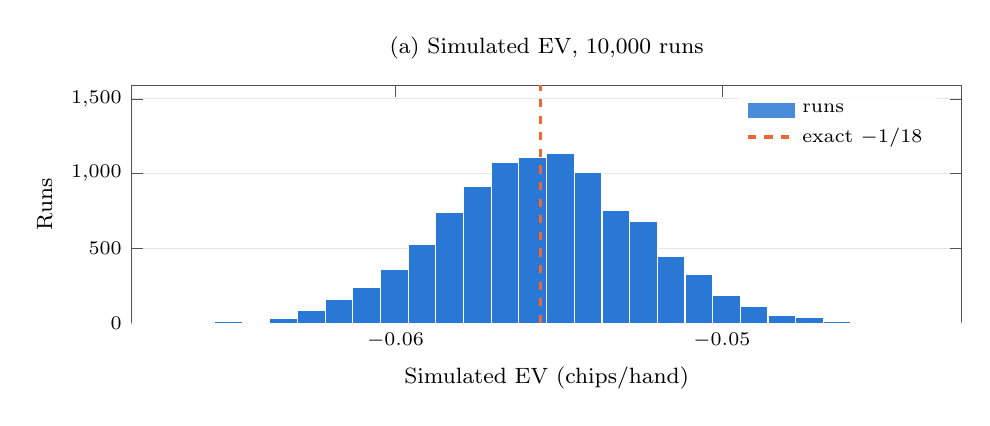
\begin{tikzpicture}[baseline=(current axis.north)]
\begin{axis}[
  width=\linewidth, height=4.6cm,
  title={(a) Simulated EV, 10{,}000 runs},
  xlabel={Simulated EV (chips/hand)}, ylabel={Runs},
  ymin=0, ymax=1590, xmin=-0.068090, xmax=-0.042650, xtick distance=0.01,
  scaled x ticks=false,
  xticklabel style={/pgf/number format/fixed, /pgf/number format/precision=2},
  legend pos=north east,
]
\addplot[ybar interval, area legend, fill=series1, draw=white, line width=0.4pt] coordinates { (-0.068090,2) (-0.067242,1) (-0.066394,2) (-0.065546,10) (-0.064698,7) (-0.063850,31) (-0.063002,84) (-0.062154,160) (-0.061306,238) (-0.060458,359) (-0.059610,526) (-0.058762,739) (-0.057914,911) (-0.057066,1073) (-0.056218,1105) (-0.055370,1136) (-0.054522,1011) (-0.053674,752) (-0.052826,683) (-0.051978,443) (-0.051130,327) (-0.050282,182) (-0.049434,110) (-0.048586,49) (-0.047738,38) (-0.046890,12) (-0.046042,5) (-0.045194,2) (-0.044346,1) (-0.043498,1) (-0.042650,1) };
\addlegendentry{runs}
\addplot[series2, very thick, dashed] coordinates {(-0.0555556,0) (-0.0555556,1590)};
\addlegendentry{exact $-1/18$}
\end{axis}
\end{tikzpicture}
\end{minipage}\hfill
\begin{minipage}[t]{0.48\linewidth}
\centering
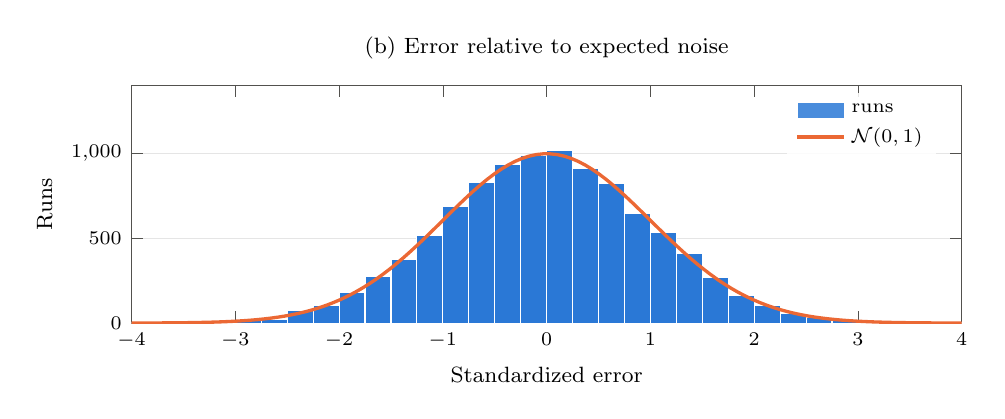
\begin{tikzpicture}[baseline=(current axis.north)]
\begin{axis}[
  width=\linewidth, height=4.6cm,
  title={(b) Error relative to expected noise},
  xlabel={Standardized error}, ylabel={Runs},
  ymin=0, ymax=1400, xmin=-4, xmax=4,
  legend pos=north east,
]
\addplot[ybar interval, area legend, fill=series1, draw=white, line width=0.4pt] coordinates { (-4.000,3) (-3.750,1) (-3.500,2) (-3.250,3) (-3.000,13) (-2.750,20) (-2.500,73) (-2.250,106) (-2.000,183) (-1.750,272) (-1.500,372) (-1.250,517) (-1.000,685) (-0.750,827) (-0.500,935) (-0.250,989) (0.000,1018) (0.250,909) (0.500,821) (0.750,645) (1.000,534) (1.250,411) (1.500,269) (1.750,161) (2.000,104) (2.250,59) (2.500,36) (2.750,17) (3.000,11) (3.250,2) (3.500,1) (3.750,1) (4.000,1) };
\addlegendentry{runs}
\addplot[series2, very thick, domain=-4:4, samples=120] {10000*0.25*exp(-x^2/2)/sqrt(2*pi)};
\addlegendentry{$\mathcal{N}(0,1)$}
\end{axis}
\end{tikzpicture}
\end{minipage}
\caption{(a) Simulated EV of all 10{,}000 runs ($M = 200{,}000$ hands each);
the dashed line is the exact value $-1/18$. (b) Each run's error divided by its
expected size, compared with a standard bell curve.}
\label{fig:sim}
\end{figure}

\begin{table}[htb]
\centering
\small
\caption{Simulated EV ($M = 200{,}000$ hands per run) compared with the exact
EV of $-1/18 = -0.0555556$, over 10{,}000 runs.}
\label{tab:dev}
\setlength{\tabcolsep}{4pt}
\begin{tabular}{lr}
\toprule
Mean simulated EV & $-0.0555564$ \\
Typical error (RMS) & $0.0030$ (5.4\%) \\
Average absolute error & $0.0024$ (4.3\%) \\
Largest error & $0.0129$ (23\%) \\
Runs within 1 / 5 / 10\% & 14.6 / 64.4 / 93.3\% \\
Runs above / below $-1/18$ & 50\% / 50\% \\
\bottomrule
\end{tabular}
\end{table}

Table~\ref{tab:dev} and Figure~\ref{fig:sim} compare the simulations with the
exact value. On average the simulation is essentially perfect: over all
$2\times10^9$ simulated hands the mean is $-0.0555564$, against a true value
of $-0.0555556$. Single runs miss by about $0.003$ (5\%), which is exactly the
error we expect from $M = 200{,}000$ random hands: each hand swings by about
$1.35$ chips, and $1.35/\sqrt{M} \approx 0.003$. When each error is divided by
its expected size, the errors follow a standard bell curve
(Figure~\ref{fig:sim}b). The gap between simulated and exact EV is therefore
just sampling noise.

\section{Stage 1: learned strategies}
\label{app:strategy}

\begin{table}[htb]
\centering
\small
\caption{\peter's learned probabilities over 10{,}000 runs, compared with the
equilibrium (Eq.~\ref{eq:equilibrium}). A uniform random number has mean
$0.5$ and SD $0.29$.}
\label{tab:params}
\begin{tabular}{lccl}
\toprule
Probability & Mean & SD & Equilibrium \\
\midrule
\code{bet\_J}  & 0.505 & 0.287 & $\alpha \in [0, 1/3]$ \\
\code{bet\_Q}  & 0.000 & 0.000 & $0$ \\
\code{bet\_K}  & 0.498 & 0.288 & $3\alpha$ \\
\code{call\_Q} & 0.501 & 0.286 & $\alpha + 1/3$ \\
\bottomrule
\end{tabular}
\end{table}

\begin{figure}[tb]
\centering
\begin{minipage}[t]{0.48\linewidth}
\centering
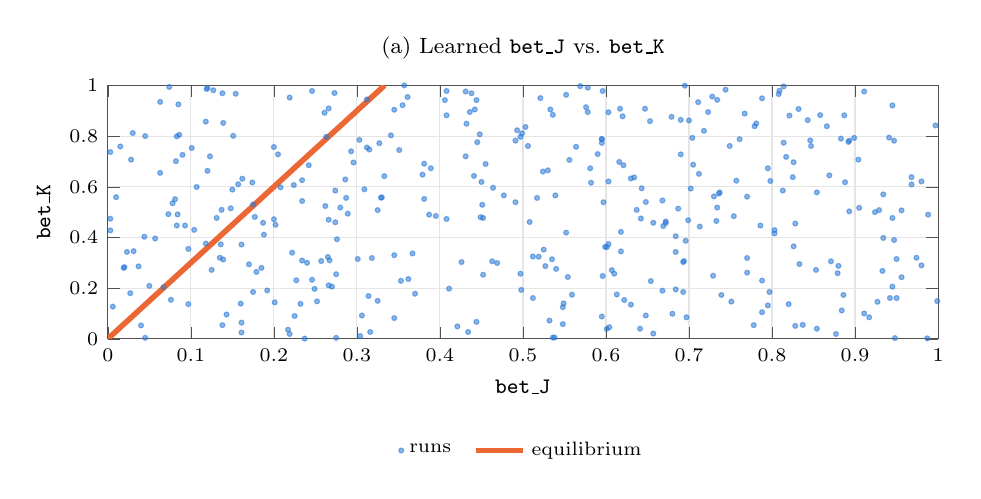
\begin{tikzpicture}[baseline=(current axis.north)]
\begin{axis}[
  width=\linewidth, height=4.8cm,
  title={(a) Learned \code{bet\_J} vs.\ \code{bet\_K}},
  legend columns=2, legend style={at={(0.5,-0.36)}, anchor=north, /tikz/every even column/.append style={column sep=6pt}},
  xlabel={\code{bet\_J}}, ylabel={\code{bet\_K}},
  xmin=0, xmax=1, ymin=0, ymax=1, xmajorgrids,
]
\addplot[only marks, mark=*, mark size=0.9pt, color=series1, fill opacity=0.55, draw opacity=0.55] coordinates { (0.444,0.942) (0.084,0.491) (0.086,0.805) (0.312,0.945) (0.293,0.74) (0.28,0.518) (0.333,0.642) (0.224,0.607) (0.175,0.185) (0.325,0.15) (0.603,0.374) (0.63,0.633) (0.536,0.884) (0.406,0.942) (0.934,0.398) (0.477,0.566) (0.452,0.477) (0.803,0.416) (0.312,0.755) (0.814,0.774) (0.77,0.261) (0.101,0.753) (0.599,0.363) (0.69,0.864) (0.927,0.146) (0.73,0.562) (0.506,0.761) (0.185,0.28) (0.669,0.445) (0.161,0.064) (0.327,0.772) (0.304,0.011) (0.647,0.908) (0.175,0.53) (0.888,0.618) (0.187,0.458) (0.61,0.257) (0.54,0.276) (0.451,0.529) (0.445,0.776) (0.286,0.629) (0.924,0.5) (0.497,0.797) (0.744,0.983) (0.781,0.85) (0.143,0.096) (0.911,0.976) (0.637,0.509) (0.843,0.863) (0.345,0.33) (0.595,0.788) (0.7,0.862) (0.974,0.32) (0.905,0.517) (0.432,0.849) (0.911,0.1) (0.107,0.599) (0.648,0.092) (0.887,0.882) (0.95,0.315) (0.361,0.954) (0.464,0.596) (0.828,0.455) (0.154,0.967) (0.123,0.72) (0.275,0.004) (0.234,0.544) (0.246,0.978) (0.968,0.638) (0.499,0.811) (0.081,0.551) (0.737,0.578) (0.438,0.969) (0.814,0.996) (0.62,0.878) (0.576,0.914) (0.085,0.925) (0.246,0.233) (0.893,0.503) (0.267,0.31) (0.234,0.309) (0.202,0.45) (0.739,0.173) (0.289,0.494) (0.693,0.303) (0.987,0.002) (0.083,0.799) (0.858,0.883) (0.718,0.821) (0.997,0.842) (0.945,0.921) (0.05,0.209) (0.668,0.19) (0.019,0.28) (0.234,0.626) (0.684,0.195) (0.788,0.949) (0.712,0.651) (0.276,0.393) (0.093,0.447) (0.98,0.29) (0.045,0.8) (0.205,0.728) (0.063,0.655) (0.88,0.288) (0.09,0.726) (0.345,0.904) (0.351,0.745) (0.734,0.943) (0.729,0.249) (0.33,0.558) (0.751,0.147) (0.696,0.387) (0.357,1.0) (0.795,0.132) (0.767,0.889) (0.797,0.185) (0.219,0.952) (0.595,0.773) (0.078,0.535) (0.728,0.956) (0.057,0.396) (0.118,0.376) (0.813,0.585) (0.578,0.895) (0.832,0.907) (0.083,0.447) (0.135,0.32) (0.552,0.963) (0.24,0.3) (0.617,0.908) (0.668,0.546) (0.803,0.429) (0.672,0.463) (0.809,0.979) (0.273,0.97) (0.455,0.69) (0.12,0.663) (0.69,0.728) (0.828,0.051) (0.521,0.95) (0.367,0.337) (0.015,0.759) (0.788,0.23) (0.266,0.47) (0.533,0.905) (0.68,0.099) (0.654,0.228) (0.503,0.836) (0.817,0.718) (0.118,0.857) (0.945,0.477) (0.067,0.204) (0.734,0.518) (0.618,0.422) (0.345,0.082) (0.934,0.57) (0.846,0.783) (0.569,0.997) (0.263,0.797) (0.657,0.021) (0.023,0.343) (0.596,0.248) (0.15,0.589) (0.641,0.04) (0.854,0.578) (0.003,0.737) (0.2,0.757) (0.217,0.036) (0.389,0.673) (0.275,0.255) (0.947,0.782) (0.01,0.559) (0.296,0.696) (0.37,0.178) (0.548,0.058) (0.262,0.524) (0.097,0.137) (0.341,0.803) (0.884,0.112) (0.879,0.259) (0.137,0.509) (0.77,0.561) (0.232,0.138) (0.441,0.643) (0.138,0.969) (0.786,0.447) (0.788,0.105) (0.833,0.295) (0.411,0.198) (0.702,0.593) (0.442,0.905) (0.265,0.323) (0.491,0.539) (0.821,0.881) (0.564,0.758) (0.082,0.701) (0.161,0.025) (0.395,0.485) (0.597,0.539) (0.266,0.211) (0.355,0.922) (0.139,0.852) (0.2,0.472) (0.222,0.34) (0.904,0.707) (0.426,0.303) (0.854,0.04) (0.705,0.687) (0.933,0.268) (0.711,0.934) (0.381,0.552) (0.653,0.859) (0.77,0.319) (0.679,0.876) (0.434,0.027) (0.274,0.585) (0.621,0.685) (0.778,0.054) (0.266,0.909) (0.325,0.508) (0.559,0.174) (0.948,0.003) (0.657,0.458) (0.723,0.895) (0.408,0.882) (0.687,0.514) (0.866,0.839) (0.512,0.161) (0.448,0.807) (0.837,0.055) (0.493,0.823) (0.554,0.244) (0.98,0.621) (0.877,0.019) (0.219,0.019) (0.188,0.411) (0.287,0.556) (0.601,0.362) (0.779,0.839) (0.03,0.812) (0.353,0.229) (0.037,0.286) (0.073,0.492) (0.548,0.125) (0.601,0.039) (0.179,0.264) (0.929,0.508) (0.883,0.79) (0.449,0.48) (0.12,0.99) (0.757,0.624) (0.53,0.665) (0.138,0.054) (0.301,0.315) (0.497,0.257) (0.463,0.306) (0.988,0.49) (0.871,0.306) (0.249,0.197) (0.362,0.236) (0.498,0.193) (0.604,0.046) (0.642,0.475) (0.148,0.515) (0.225,0.09) (0.736,0.573) (0.733,0.465) (0.556,0.706) (0.16,0.139) (0.761,0.788) (0.309,0.59) (0.192,0.191) (0.136,0.373) (0.549,0.14) (0.408,0.473) (0.693,0.185) (0.942,0.161) (0.517,0.556) (0.252,0.148) (0.028,0.707) (0.603,0.894) (0.695,0.999) (0.261,0.892) (0.968,0.609) (0.538,0.005) (0.672,0.457) (0.161,0.372) (0.613,0.175) (0.899,0.793) (0.552,0.419) (0.536,0.005) (0.003,0.428) (0.508,0.461) (0.201,0.144) (0.242,0.685) (0.684,0.405) (0.318,0.319) (0.519,0.324) (0.648,0.54) (0.524,0.66) (0.956,0.243) (0.45,0.619) (0.917,0.085) (0.27,0.206) (0.227,0.231) (0.131,0.477) (0.157,0.61) (0.097,0.355) (0.003,0.474) (0.315,0.747) (0.82,0.137) (0.795,0.673) (0.174,0.617) (0.044,0.403) (0.947,0.39) (0.17,0.294) (0.826,0.697) (0.59,0.729) (0.634,0.637) (0.006,0.127) (0.379,0.648) (0.578,0.991) (0.622,0.153) (0.853,0.272) (0.798,0.623) (0.616,0.698) (0.469,0.299) (0.491,0.782) (0.595,0.788) (0.532,0.072) (0.704,0.793) (0.314,0.169) (0.893,0.782) (0.031,0.346) (0.699,0.468) (0.208,0.598) (0.941,0.794) (0.274,0.46) (0.162,0.632) (0.125,0.272) (0.754,0.484) (0.444,0.067) (0.063,0.935) (0.316,0.027) (0.431,0.72) (0.643,0.594) (0.956,0.507) (0.945,0.206) (0.582,0.616) (0.076,0.154) (0.808,0.966) (0.749,0.761) (0.452,0.253) (0.119,0.986) (0.303,0.785) (0.713,0.443) (0.045,0.004) (0.139,0.313) (0.527,0.287) (0.421,0.049) (0.603,0.621) (0.999,0.149) (0.436,0.895) (0.408,0.978) (0.684,0.343) (0.387,0.49) (0.826,0.365) (0.151,0.801) (0.381,0.691) (0.525,0.352) (0.257,0.307) (0.306,0.092) (0.512,0.325) (0.607,0.271) (0.074,0.994) (0.63,0.135) (0.618,0.345) (0.02,0.283) (0.329,0.557) (0.847,0.761) (0.886,0.173) (0.596,0.978) (0.581,0.673) (0.104,0.43) (0.825,0.638) (0.431,0.976) (0.697,0.085) (0.04,0.053) (0.177,0.481) (0.869,0.645) (0.535,0.314) (0.127,0.981) (0.539,0.566) (0.95,0.161) (0.595,0.088) (0.694,0.307) (0.027,0.18) (0.892,0.777) (0.237,0.001) };
\addlegendentry{runs}
\addplot[series2, line width=2pt] coordinates {(0,0) (0.33333,1)};
\addlegendentry{equilibrium}
\end{axis}
\end{tikzpicture}
\end{minipage}\hfill
\begin{minipage}[t]{0.48\linewidth}
\centering
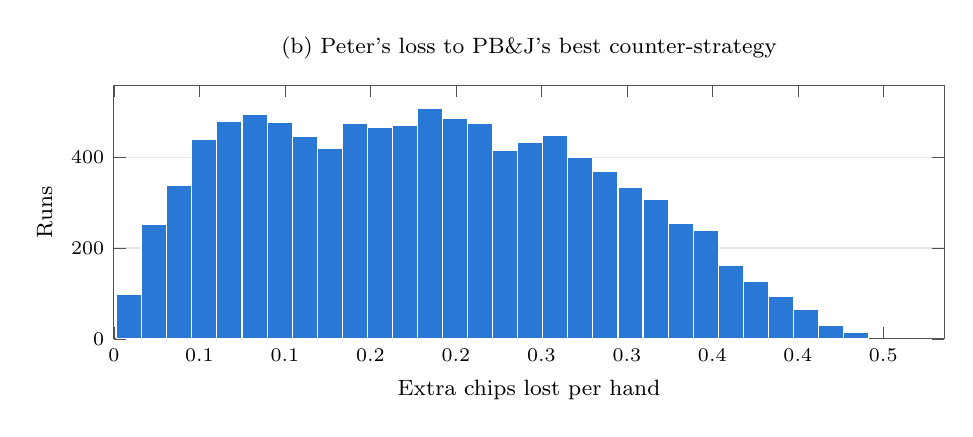
\begin{tikzpicture}[baseline=(current axis.north)]
\begin{axis}[
  width=\linewidth, height=4.8cm,
  title={(b) \peter's loss to \pbj's best counter-strategy},
  xlabel={Extra chips lost per hand}, ylabel={Runs},
  ymin=0, xmin=0,
  scaled x ticks=false,
  xticklabel style={/pgf/number format/fixed, /pgf/number format/precision=1},
]
\addplot[ybar interval, fill=series1, draw=white, line width=0.4pt] coordinates { (0.00161,98) (0.01627,251) (0.03093,337) (0.04559,439) (0.06026,479) (0.07492,494) (0.08958,477) (0.10424,445) (0.11890,420) (0.13356,475) (0.14822,465) (0.16288,469) (0.17754,507) (0.19221,485) (0.20687,474) (0.22153,414) (0.23619,432) (0.25085,448) (0.26551,399) (0.28017,368) (0.29483,334) (0.30949,307) (0.32416,253) (0.33882,238) (0.35348,162) (0.36814,127) (0.38280,94) (0.39746,65) (0.41212,30) (0.42678,14) (0.44144,14) };
\end{axis}
\end{tikzpicture}
\end{minipage}
\caption{(a) Learned \code{bet\_J} against \code{bet\_K} for 400 random runs.
At equilibrium every point would lie on the orange line
($\code{bet\_J} = \alpha$, $\code{bet\_K} = 3\alpha$). (b) How much more each
learned strategy would lose if \pbj{} switched to its best counter-strategy
(0 for an equilibrium strategy).}
\label{fig:strategy}
\end{figure}

\end{document}
